\documentclass[11pt,a4paper]{article}
\usepackage[T1]{fontenc}
\usepackage{graphicx}
 \usepackage[latin1]{inputenc}
\setlength{\topmargin}{-.5in}
\setlength{\textheight}{9in}
\setlength{\oddsidemargin}{.125in}
\setlength{\textwidth}{6.25in}
\begin{document}
\title{Parallel Algorithms Coursework}
\author{C\'edric DESSEZ, Valentin GRAND, Yann NICOLAS, Cyril NOVEL, Nicolas SERVEL}
\maketitle

\section{Gathering the clues}
The first thing we did was to analyse in depth the evidence given by our intel. Hopefully the engineers from Nukehavistan were kind enough to leave clues about the computer system.

The very first thing we did was to find the identity of the man portrayed on the system. We were able to process the face into the database of Interpol, hoping we will find a rogue scientist working for the Nukehavistan. Unfortunately no match were found. We then used the ReverseImages tool Q made for us and found that the man was \textit{Leonhard Euler}, portrayed on a 1957 stamp of the USSR. Such a link supposes that the Nukehavistan is a communist nation and so a major threat to the democracy all around the world.

Because of the link with the USSR, we assumed that the funny writing above the clock was in Cyrillic script. As no one in our team was able to understand russian, we contacted the Translation Service of the MI-6. The translation was \textit{fast inverter integrated functions}.

The text below the clock is in french. As we are french, we perfectly understood it and it means \textit{Made in France}. However, it is very unlikely this machine was produced in France. The final design is ugly and everyone knows French are all about beauty and class. We assumed this was only a trick to harden our research.

\begin{figure}[!h]
\centering
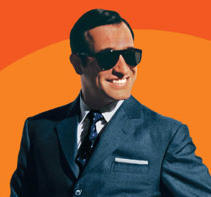
\includegraphics[width=5cm]{oss.png}
\caption{The model of the classy French spy}
\label{frenchspy}
\end{figure}

We then took a look to the two sets of coordinates. The set along the board points to the lovely village of \textit{Beaumont-en-Auge} in France. Among the famous people born in this town, one stands out. \textit{Pierre Simon de Laplace} was a mathematician and his work could have highly interested the Nukehavistan. The second coordinates confirmed our idea : it points near the \textit{Laplace} RER station in Paris. We don't believe in coincidence. Laplace's work is the key of the system. The power to the minus one on the second set of coordinates strengthens our assumption about the \textit{inverter}.

We finally called the technical hotline. Since it is a charged number, we joined the bill at the end of the report. The technical hotline is only an answerbot. We tested if it was telling the truth by asking it the answer to the Ultimate Question of Life, the Universe and Everything. Since it answered 42, we assumed the bot was powerful enough to answer our upcoming questions\footnote{This raises serious issues about the advanced level of Nukehavistan in the Computer Science field. Maybe we should applied for a PhD in their university.}. When we asked what was in the box, it said \textit{Numerical Inversion of Laplace Transforms of Probability Distributions}. A quick and efficient DuckDuckGo search -- we made sure we weren't tracked -- pointed us to a research paper from 1995, presenting an algorithm using the Euler method for inverting Laplace transforms.

The loop was almost complete. We knew what the algorithm was and what to code. The only thing we didn't know was what the program was actually doing. We tried to reverse engineer the \textit{mystery.o} file. We obtained some strange figures.

\begin{figure}[!h]
\centering
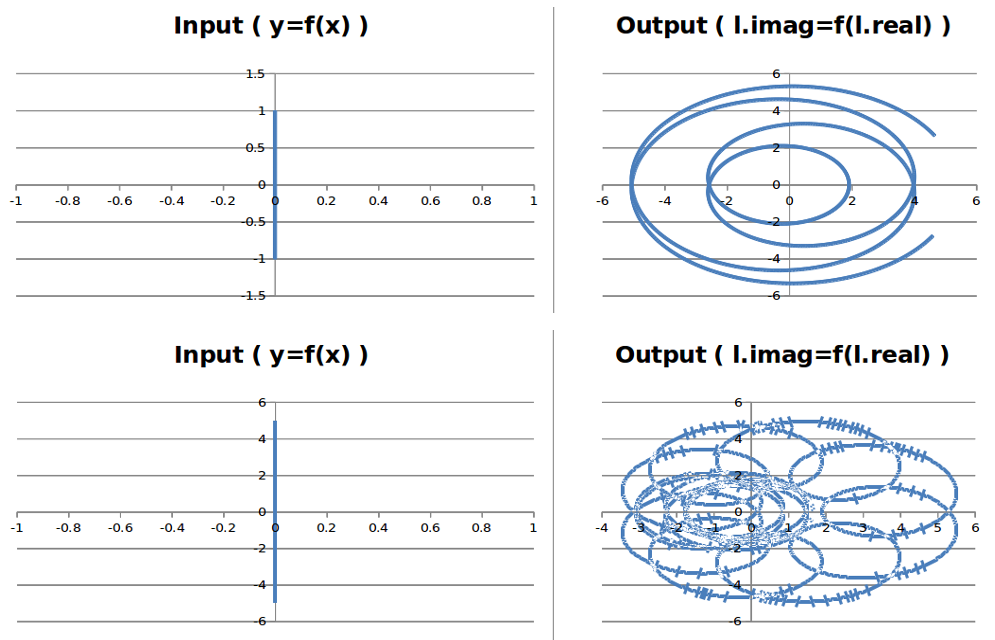
\includegraphics[width=10cm]{outputs.png}
\caption{Reverse engineering inputs and ouptuts.}
\label{reverse}
\end{figure}

We then made two assumptions. The first possibility is that the Nukehavistan is trying to communicate with superior life forces. The second possibility is that this computer system is prime in the job of the Nukehavistan spies. Since we are fierce scientists, we ruled out the first option. Thus we brainstormed over the second option by watching all the James Bond movies. At the end of this intensive marathon, we reached a conclusion :

\begin{figure}[!h]
\centering
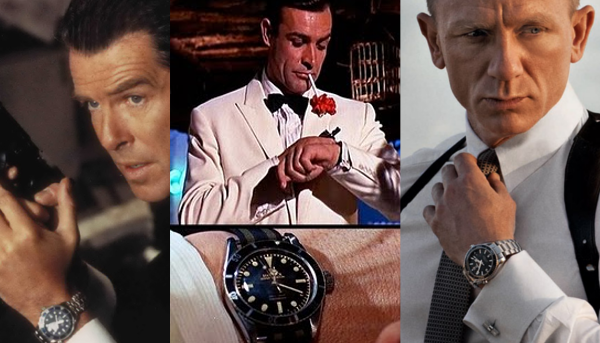
\includegraphics[width=8cm]{watches.png}
\caption{Watches}
\label{reverse}
\end{figure}

Every spy needs a good watch! If we look closely to the computer system, the small peak of the output is on the 3 and the big peak is on the 11. The clock has its small hand pointing between 3 and 4 -- so in the 3 \textsuperscript{rd} hour. The large hand is pointing at 11. So the output of the computer system gives us the time!

\section{Implementation}

\subsection{Sequential algorithm}

\subsection{Parallel MPI algorithm}

\subsection{Parallel OpenMP algorithm}

\end{document}
